\section{The Self-Sovereign Data Economy}  % TODO title change

% General overview defining data as an asset, actors in data economy, and how SDL can expand 

In this section we will define data as an asset class, explain the utility of data, and define the actors in the self-sovereign data economy. We will also provide a cursory analysis of the actors within the Snickerdoodle protocol, and how they assume the roles defined here.

\subsection{Data as an Asset}
% Data has value and can be treated as an asset. How is it different/similar to traditional assets
% https://money.cnn.com/news/newsfeeds/articles/stocktwits/pointsandfigures_9937.html?iid=EL#:~:text=Commodities%20are%20assets%2C%20but%20unlike,can%20derive%20out%20of%20them.
In an information economy, data is the most fundamental commodity there is. In order to understand the individualized data economy, we must highlight the difference between assets and commodities. While commodities are an asset class, they have unique properties. Unlike most other asset classes, commodities are traded at high volume. While it is possible to purchase small volumes of commodities, they are often illiquid due to the markets operating at high volumes. While fractional vehicles like ETFs do exist, these are fundamentally not equivalent, as they represent nothing more than a symbolic debt obligation and not the resource itself. As an example, it is possible to buy an individual gallon of oil, but much harder to sell it as the markets do not trade oil by the gallon. Conversely, it is much easier to sell a thousand barrels of the same oil since the commodities markets trade at these quantities regularly. In much the same way, individual data is not valuable in today's data economy, and it is almost exclusively traded in the aggregate.

There are cases in which individualized markets have developed around commodities. For example, in the wake of the 2008 financial crisis, consumers rushed to purchase gold as trust in financial assets, currencies, and markets plummeted. Nations and banks often trade in gold in large quantities, and as a result gold markets trade in units ranging from the thousands to the millions. In order to facilitate the liquidity of consumer gold, a number of gold purchasing operations have sprung up in order to provide liquidity to the individual and aggregate gold for commodities markets. Because of the non-triviality of data ownership (see below), this infrastructure has yet to be created for data. This is what the Snickerdoodle protocol aims to enable.


\subsubsection{Utility of Data}
% What can we do with data

% What is the value of data 
%.      How can people get value
%       How can businesses get value

Data provides so much utility in the twenty first century and revolutionized every industry. From supply chain, to medicine, to biotech, to sports, to self driving cars. Some of this involves some insane computing such as using machine learning to generate humans faces and entire paragraphs to less complex tasks like finding the quickest route home. There is also a dark side to this as all this data allows for complex and automated ways to track people. (MORE CITATIONS). 

\subsubsection{An individual's role in the data economy} 
%TODO moving this to the top bc I think it'll help if flow better -- not sure where on the top it fits the best
% What is the role of an individual right now?
% Looking at the flow how can an individual's role be expanded
The problem with the current data economy is that the individual that is generating the data doesn't have control over how their data is being used and isn't being properly compensated for their role in the data economy. Different governments are recognizing the need to give users control such as the GDPR and CCPA (CITE THINGS + maybe more info). While the data economy is said to be valued around XXX at the time of writing (CITE), individuals aren't getting their fair share of this pie. (NEED MORE CITATIONS -- maybe Kara Swisher cheap date, also need harder sources). 
\newline
\newline
Another problem is that the lack of ownership / control of data leads to ways for governments to get around surveillance laws. Instead of having to get a warrant to view individual data, governments can buy the data from data brokers (CITE). This creates a opaque way for governments to spy on individuals. An example of this is the US government's ICE agency created a large data base through publicly available information and data brokers that allows them to track everyone in the US without a warrant (CITE). 

\subsubsection{Data Ownership}
% How can individuals control / own their data
The Snickerdoodle protocol aims to shift the balance of power within the existing data economy by providing individuals greater control of their data. In order to do so we must first understand value within the existing data economy and what it means to control and own data. While many attempts have been made to codify control of data through legislative means (GDPR, etc.), we will attempt to provide a technical definition here.

% The goal of this protocol is to maintain the value in the current data economy while flipping the power structure on its head by giving individuals control of the data they generate. This is consistent with the trend we see in modern legislation (CONTINUE TO GIVE CONTEXT).

Ownership of data is a difficult concept to define. Unlike physical resources, data can be copied indefinitely, is generated constantly, and generally requires technical expertise and infrastructure for collection and value extraction. Additionally, these properties make regulating the use of data inherently difficult.

To illustrate these properties let us use the example of Alice: a customer shopping at a grocery store. By simply being at the store, Alice has generated data about which store she shopped at and when. When she checks out, she is generating data about what products she has bought and what payment method she used. When she leaves she has generated data about how long she was in the store. All of this data may have value, and a number of actors may be collecting it. The store may be collecting this data through surveillance and/or loyalty programs. Her phone may have software collecting her location data. Her credit card company may be tracking her spending habits. In the existing data economy, these entities performing the collection have total sovereignty in how the data is used. They may analyze this data for targeted advertising, perform market research, or even sell it to other parties. In addition, all of these actions may be taken with no expected standard of privacy, security, or anonymity for Alice. Alice is not likely to have knowledge about what data was collected, who collected it, who has access to it, or how it is being used. She is also not compensated for the value that is extracted from this data, despite the fact that she is the one who originated it.

% For example imagine if Alice walks into a store to buy some goods. She's now generated data about where/when she was, what goods she's bought, how long she spent in the store, and what type of payment method she's used. Does the store get to know all of this? Does her cell phone or apps on her phone get to know? Are they allowed to know that it's Alice? What are they allowed to do with the data? Can they try to optimize for what goods to buy or give an app notification of a discount? Are they allowed to sell this data to others who are interested in tracking people's movements? What if the store is now a pharmacy giving a prescription? What if the data gets leaked? What does Alice think about this whole exchange? %TODO clean up but like the idea

%        Define what owning data mean
In the above example, the concerns around collection and privacy are immediately apparent, but this example also brings into question what it actually means to own data. In Alice's case, her data is being collected by third parties who may then sell or exchange it with other parties. Due to the infinite duplicability of digital data, any such exchange results in both parties possessing the data. In this case who actually owns the data? Is it the party that collected it? Is it collectively owned by all parties that are currently storing it? Or is it owned by the party that originated it (Alice)? In the existing model, data is owned by the entities that store it, and may be legally attributable to the entity that collected it (CITE). In our context, we define data ownership as follows:

\begin{definition}
\label{definition:DataOwnership}
Data Ownership: If an individual can exclusively control and manage the collection, storage, and usage of a piece of data in a secure and private manner, then it can be said that they own it.
\end{definition}

In the case of data, privacy and security are critically important since compromised data is no longer self-sovereign. If another party has gained access to the data, it is virtually impossible to maintain data ownership as exclusivity has been lost. This is why the Snickerdoodle Protocol aims to provide privacy and security through the exchange of data insights rather than the exchange of data itself. Additionally, the management of the data should be made easy to the user.

% Due to how tricky it is to define data ownership, our protocol focuses on allowing users to control data they they generate. Specifically we want to enable a protocol that gives users to safely managed how their data is collected, stored, and shared. Additionally, parties that are interested in subscribing to individual's data can do so without compromising the safety of that data. The protocol should also maintain the authenticity and interoperability of data to ensure that the data being process is valid and usable.

%        How technically they can do this -- Introduce data wallet

%  Data asset life cycle
% collect/store/share/manage/own

\subsection{Important Properties of Data}
The goal of the Snickerdoodle Protocol is to enable all the benefits of the current data economy while allowing individuals to own their data. This means individuals should be able to control and manage how their data is collect, stored, and shared (?used?). 

\subsubsection{Privacy}
Privacy of data boils down to who is able to know what about about the data. For example, who gets to know what an individual's management settings are and who gets to know where the data was collected from and stored. The trickiest part of privacy is maintain privacy after the data has been shared with other parties. If Alice shares her location data $D$ with Bob, privacy is maintained if Bob can't figure out that $D$ belongs to Alice. Controlling who is allowed to know what about the data also extends to metadata created and allowing the owners of the data to be able to delete they want to be deleted. 

\subsubsection{Security}
Security of data and the protocol mean that only authorized entities are allowed to interact with the data and the protocol works in the intended way. Only people with the correct keys should be able to manage consent and share data. Data in storage and in transit should always be encrypted. Forward and backwards secrecy should be maintained. The protocol and all tools to interact with the protocol should be updatable so vulnerable bugs should be patched. Additionally, it should be easy for people to use the best security practices possible.

\subsubsection{Interoperability}
The data within the system should be interoperable, or easy for everyone to use. It should be easy to compute for data that's collected from multiple sources and stored on different services. One way this can be achieved is through open sourced data schemas that are stored with the data (DO WE WANT TO CITE A SECTION). Additionally, it should be possible for multiple different software providers to make a management software that works with the system and the management software should be able to integrate easily with different identity providers (in the Snickerdoodle Protocol this management software is a data wallet -- see section \ref{section:DataWallet}).

\subsubsection{Authenticity}
The data in the system should be authentic, or easy to validate its accuracy. For example, if Alice is trying to prove that she's over 21 to Bob's Bar, Bob should be able to confirm that her age Data came from the California DMV. The system needs to make sure that information related to authenticity is safely transferred as it is collect, stored, and shared. It's worth highlighting that authenticity and privacy can often come at odds (e.g., when Alice revealed her age she revealed she lived in California recently enough to get a driver's licence). 


\subsection{Actors in the Data Economy}
\label{section:Actors}
% TODO should we define verified and unverified data?
% Who is involved in the data economy
%.    Break down into personas
%.    Break down how data flows

The data economy is a complex system that collects data on individuals, moves the data around, and runs some analysis on that data. In this section we will break down the different actors within the system and explain how they interact.


%TODO overview of everything
Within the data economy the $data\ owner$ generates data in some manner. A $data\ subscriber$ is interested in the data generated by that owner and a subset of all other owners generating data. In order for the this to happen a $data\ collector$ collects the data generated and stores it in a $data\ custodian$. A $data\ aggregator$ then aggregates all of the data and advertises its ownership of the data. The subscriber is interested in some insight so they pay to run a $data\ application$ on the aggregated data. This payment flows back through the economy. This flow can be seen in figure \ref{fig:DataActors}.  Please note, a multiple actors can be represented by a single entity (e.g., Google collects data, stores data, aggregates data, and runs analysis on the data).

In order for this to be a self-sovereign data economy the data owner must actual own the data and thus be in control of how it is used. This means that the owner must be able to manage the collectors and custodians of their data and be able to control who aggregates and shares their data. Additionally payment must be distributed equitably to the parties in this economy such that the owner gets their fair share and all the actors have an incentive to behave.

\begin{figure*}[!htbp] 
    \centering
    % \textbf{a.}
    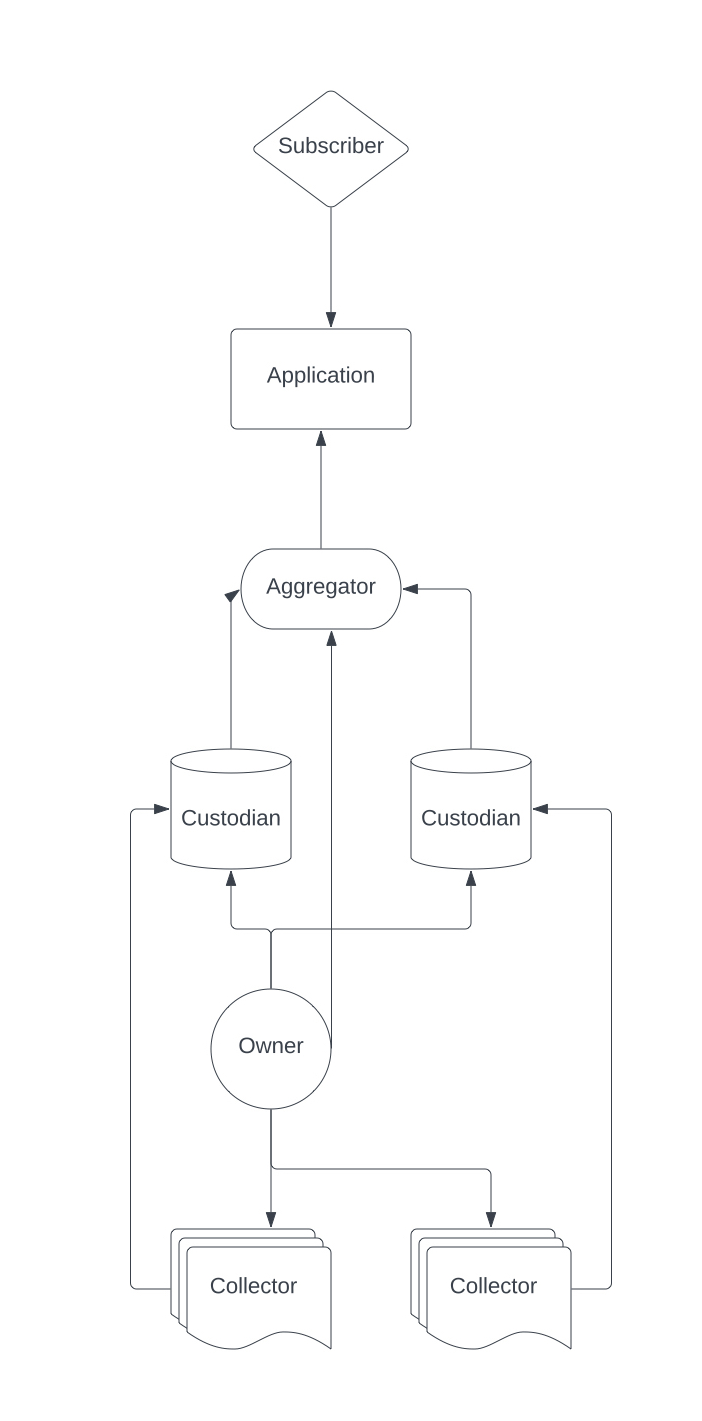
\includegraphics[width=170]{images/persona_strucutre.jpg}
    \caption{The flow of data in the data economy. The data is generated by the owner and flows from collectors to custodians to aggregators to applications and finally to the subscriber. The subscriber pays money that trickles back through the system. In order for the owner to actually have ownership of their data they must be able to manage the collector, custodian, and aggregator of their data.}
    \label{fig:DataActors}
\end{figure*}


\subsubsection{Data Owner}
A data owner is the person who generates the data and, in a system that empowers the individual, would be able to control/own their data as defined by definition \ref{definition:DataOwnership}. The identity of the owner is represented by a set of cryptographic keys and these keys would enable the individual to manage their data. This identity may or may not be anonymous.
\newline
\newline
Being able to control your identity is key to being able to control data tied to your identity. This is where the ability to create and control a Decentralized Identifier (DID) is central to individual data sovereignty. 
% Should we find a way to tie this to the data wallet section or future 

\subsubsection{Data Subscriber}
Data subscribers are the entities interested in leveraging user data. These are the businesses and other organizations that provide compensation in exchange to access for data. A system that preserves individual ownership and keeps user data safe would only allow subscribers to access to anonymized data or through compute-to-data processes.
\newline
\newline
The fundamental role of the Snickerdoodle Protocol would be to facilitate this exchange in safe way. 

\subsubsection{Data Aggregators}
Data aggregators allow individuals to share data with interested subscribers and usually pool individuals together to improve the utility of the data. They can also be though of a data pool or a data cooperative that helps match buys and sellers of data-based assets.
\newline
\newline
Making sure that data aggregators can facilitate this exchange in a safe way is key to enabling a self sovereign data economy and is fundamental problem the Snickerdoodle Protocol aims to solve.

\subsubsection{Data Custodian}
Data custodian's store data on behalf of the data owners. To enable individual data ownership this storage needs to be safe. In order for this to be done in a trustless manner, a proof model capable of proving both storage and deletion will become necessary. Additionally any protocol trying to enable a self sovereign data economy, including Snickerdoodle, needs to create an incentivization scheme to make sure data custodians don't have an incentive to sell data directly to data subscribers.

\subsubsection{Data Collectors}
Data collectors are the entities that collect user data and are the data on-ramp to the system. They are the originator of the data assets and their schemas. It is worth reiterating that collectors are not necessarily distinct from custodians and may be the same entity; however, owners may choose to have their data collected by one entity and stored with another. Similarly to custodians, collectors should also be incentivized to not directly give data to subscribers.

\subsubsection{Data Application}
Data applications process data to provide insights to subscribers. It's worth pointing out that this data application can be created by anyone such as the subscriber, the aggregator, or a third party. Regardless of the entity that owns/acts as a data application in order to create a self-sovereign data economy the data application can't compromise the data it's processing. In addition to the safety guarantees, individuals need to be able to give informed consent to the data application. In order for this to happen the data application needs to make clear what data is going to be processed and what the insight is going to be used for.


\subsection{Actors in Version 1}
% For our version 1 how are we going to break down the actors/personas
%     Individual's / end users
%.    Businesses
%     DAO
%.    SDL
For version 1 of the Snickerdoodle Protocol we are going to simplify the actors in order to build a working system that allows individuals to control their data. For version 1 there will be 4 actors: $Individuals$, $Businesses$, the $Snickerdoodle\ DAO$, and $Snickerdoodle\ Insight\ Service$. 
Individuals are the owners that will install a data wallet that will help individuals (see section \ref{section:DataWallet}). The data wallet will act as a collector and custodian by collecting and storing information locally for the individual. 
Businesses are the subscribers and the Snickerdoodle Insight Platform will help them create data applications through use of the Snickerdoodle Query Language (see sections \ref{section:InsightService} and \ref{section:SDQL} for more info on the Insight Platform and query language respectively).
The Snickerdoodle DAO will provide a decentralized way to manage the protocol (see \ref{section:DAO}). Part of this includes the creation of on-chain consent contracts. These contracts act as data aggregators by allow individuals to consent to sharing their data with a businesses (see section \ref{section:ConsentContract}).

For implementation details check out section \ref{section:Implementation} and for ways we'll expand V1 check out section \ref{section:Future}.
